\documentclass{article}
\usepackage{amsmath} % For matrix environments and math tools
\usepackage{tikz} % For drawing circles and annotations
\usetikzlibrary{matrix}
\title{Matrix in LaTeX Tutorial}
\author{MMADUs}
\date{\today}

\begin{document}

\maketitle

\section{Matrix Environments}

\subsection{1. Matrices with Parentheses (pmatrix)}
\[
A = \begin{pmatrix}
1 & 2 & 3 \\
4 & 5 & 6 \\
7 & 8 & 9
\end{pmatrix}
\]

\subsection{2. Matrices with Square Brackets (bmatrix)}
\[
B = \begin{bmatrix}
1 & 2 & 3 \\
4 & 5 & 6 \\
7 & 8 & 9
\end{bmatrix}
\]

\subsection{3. Matrices with Braces (Bmatrix)}
\[
C = \begin{Bmatrix}
1 & 2 & 3 \\
4 & 5 & 6 \\
7 & 8 & 9
\end{Bmatrix}
\]

\subsection{4. Determinant Style Matrices (vmatrix)}
\[
D = \begin{vmatrix}
1 & 2 & 3 \\
4 & 5 & 6 \\
7 & 8 & 9
\end{vmatrix}
\]

\subsection{5. Double Vertical Bars (Vmatrix)}
\[
E = \begin{Vmatrix}
1 & 2 & 3 \\
4 & 5 & 6 \\
7 & 8 & 9
\end{Vmatrix}
\]

\subsection{6. Matrices Without Brackets (matrix)}
\[
F = \begin{matrix}
1 & 2 & 3 \\
4 & 5 & 6 \\
7 & 8 & 9
\end{matrix}
\]

\section{Marking or Highlighting Matrix Elements}

\subsection{1. Circling Specific Elements}

\begin{center}
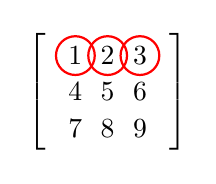
\begin{tikzpicture}
\matrix (m) [matrix of math nodes,left delimiter={[},right delimiter={]}]
{
  1 & 2 & 3 \\
  4 & 5 & 6 \\
  7 & 8 & 9 \\
};
\draw[red, thick] (m-1-1.center) circle(7pt); % Circle element (1,1)
\draw[red, thick] (m-1-2.center) circle(7pt); % Circle element (1,2)
\draw[red, thick] (m-1-3.center) circle(7pt); % Circle element (1,3)
\end{tikzpicture}
\end{center}

\textbf{Note:} Access individual cells using the syntax \texttt{m-<row>-<column>}.\

\subsection{2. Highlighting Rows or Columns}

\begin{center}
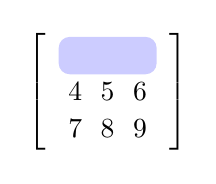
\begin{tikzpicture}
\matrix (m) [matrix of math nodes,left delimiter={[},right delimiter={]}]
{
  1 & 2 & 3 \\
  4 & 5 & 6 \\
  7 & 8 & 9 \\
};
\fill[blue!20,rounded corners] (m-1-1.north west) rectangle (m-1-3.south east); % Highlight row 1
\end{tikzpicture}
\end{center}

\textbf{Note:} Syntax highlight will be \texttt{highlight-type, from, form, to}\

\section{Aligning Matrices}

\subsection{1. Aligning Matrix Elements}
You can align the elements of a matrix manually using spacing commands. For example:

\[
G = \begin{bmatrix}
1 & 2 & 3 \\
\hspace{10pt} 4 & 5 & 6 \\
7 & \hspace{10pt} 8 & 9
\end{bmatrix}
\]

\textbf{Explanation:}\ use \texttt{hspace\{n-pt\}} to add custom horizontal space.\

\section{Matrix Operations}

\subsection{1. Transpose of a Matrix}

\[
A^T = \begin{bmatrix}
1 & 4 & 7 \\
2 & 5 & 8 \\
3 & 6 & 9
\end{bmatrix}
\]

\subsection{2. Identity Matrix}
\[
I = \begin{bmatrix}
1 & 0 & 0 \\
0 & 1 & 0 \\
0 & 0 & 1
\end{bmatrix}
\]

\subsection{3. Matrix Multiplication Example}
\[
\begin{bmatrix}
1 & 2 \\
3 & 4
\end{bmatrix}
\times
\begin{bmatrix}
5 & 6 \\
7 & 8
\end{bmatrix}
= \begin{bmatrix}
(1)(5) + (2)(7) & (1)(6) + (2)(8) \\
(3)(5) + (4)(7) & (3)(6) + (4)(8)
\end{bmatrix}
\]

\end{document}